\documentclass[a4paper]{article}

%------------------------------------------------------------
\usepackage[a4paper, total={6in, 9in}]{geometry}
\usepackage{amsmath, amssymb}
\usepackage{booktabs}
\usepackage{caption}
\usepackage{enumitem}
\usepackage{graphicx}
\usepackage{float}
\usepackage{inconsolata}
\usepackage{listings}
\usepackage{mathtools}
\usepackage{pstricks-add}
\usepackage{siunitx}
\usepackage[most]{tcolorbox}
\usepackage{tikz, pgfplots}
\usepackage{epstopdf} %converting to PDF
\usepackage{hyperref}
\usepackage{xfrac}

\usetikzlibrary{shapes.geometric}
\usetikzlibrary{arrows}

%------------------------------------------------------------
\graphicspath{{./fig/}}

%------------------------------------------------------------
\setlength{\parindent}{0in}

\lstdefinestyle{C++}{
	language=C++,
	basicstyle=\ttfamily,
	keywordstyle=\color{blue}\ttfamily,
	stringstyle=\color{red}\ttfamily,
	commentstyle=\color{green}\ttfamily,
	morecomment=[l][\color{magenta}]{\#},
	showstringspaces=false
}

%------------------------------------------------------------
\newtcblisting[auto counter]{sexylisting}[2][]{sharp corners, 
    fonttitle=\bfseries, colframe=gray, listing only, 
    listing options={basicstyle=\ttfamily,language=C++}, 
    title=Listing \thetcbcounter: #2, #1}

%------------------------------------------------------------
\lstset{language=C++,
        basicstyle=\ttfamily,
        keywordstyle=\color{blue}\ttfamily,
        stringstyle=\color{red}\ttfamily,
        commentstyle=\color{green}\ttfamily,
        morecomment=[l][\color{magenta}]{\#},
        showstringspaces=false
}
%------------------------------------------------------------
\tikzstyle{block} = [draw, fill=blue!20, rectangle, 
    minimum height=3em, minimum width=3em]
\tikzstyle{sum} = [draw, fill=blue!20, circle, node distance=1cm]
\tikzstyle{input} = [coordinate]
\tikzstyle{output} = [coordinate]
\tikzstyle{pinstyle} = [pin edge={to-,thin,black}]

%------------------------------------------------------------
\newlength{\arrow}
\settowidth{\arrow}{\scriptsize$1000$}
\newcommand*{\myrightarrow}[1]{\xrightarrow{\mathmakebox[\arrow]{#1}}}

%------------------------------------------------------------

\begin{document}
\title{ENG252 Dynamics: Practical 1}
\author{Shane Reynolds}
\maketitle

\section{Introduction}
Consider an object, on Earth's surface, being launched into the air with an initial velocity at some angle with the horizontal. This very simple motion event is best analysed by considering it in two discrete parts: the object acceleration to the initial velocity; and the subsequent trajectory once the object is airborne.

\subsection{Acceleration to initial velocity}
If forces are denoted as $\boldsymbol{F}$, acceleration as $\boldsymbol{a}$, object mass as $m$, and time as $t$, then the object's acceleration can be modelled using the standard fare of Classical Mechanics: Newton's Second Law of Motion. This is shown in equation (1).
\begin{equation}
\sum \boldsymbol{F}(t) = m \boldsymbol{a}(t)
\end{equation}

The object could be accelerated along any curvilinear path, however, for the sake of simplicity let's assume the object is accelerated along a linear path. We note that acceleration can be formally defined as:
\begin{equation}
\boldsymbol{a} = \frac{d\boldsymbol{v}}{dt}
\end{equation}

Rearranging equation (1), substituting this into equation (2) and taking the integral of with respect to $t$, from the initial time, $t_0$, to the final time, $t$, yields the following:
\begin{equation}
\int_{\boldsymbol{v_0}}^{\boldsymbol{v}(t)} d\tilde{\boldsymbol{v}} = \frac{1}{m}\int_{t_0}^{t} \sum \boldsymbol{F}(\tau) d\tau
\end{equation}

Assuming that the force is constant over the duration of time $t-t_0$, equation (3) can be simplified as follows:
\begin{equation}
\boldsymbol{v}(t) = \boldsymbol{v_0} + \frac{(t-t_0)}{m} \sum \boldsymbol{F} 
\end{equation}

If the motion is planar then equation (4) can be decomposed according to a conveniently chosen two dimensional rectilinear orthonormal basis which describes the vector space. Typically, we use $\boldsymbol{\hat{e}_x}$, and $\boldsymbol{\hat{e}_y}$, such that $\boldsymbol{\hat{e}_y}$ is aligned with the force due to gravity, but any arrangement could be used.

\subsection{Trajectory once airborne}
Once airborne, there are typically only a few forces acting on the object: force due to gravity; and force opposing motion due to friction between the object and air. The force due to gravity can be calculated using another \textit{greatest hit} from the Classical Mechanics cannon: Newton's Law of Universal Gravitation. If we denote the mass of our object as $m$, the mass of the Earth as $M$, the Euclidean distance between their centres as $r$, and $G$ as a gravitational constant $6.674×10^{−11} \si{\newton(\meter\per\kilogram)^2}$ then the attractive force due to gravity is given by:
\begin{equation}
\boldsymbol{F} = G \frac{m M}{r^2}
\end{equation}

Assuming that the object trajectory does not take large excursions from the Earth's surface it is reasonable to assume that $r$ is constant, implying that the force due to gravity is also constant. If the force due to air resistance is assumed to be negligible, then the object is said to be undermoving constant acceleration $g$, which is approximately $9.81\si{\meter\per\second^2}$. A 2D orthonormal basis describing the vector space of the motion, say $\boldsymbol{\hat{e}_x}$ and $\boldsymbol{\hat{e}_y}$, can be aligned such that $\boldsymbol{\hat{e}_y}$ is parallel to the direction of $g$. Under these assumptions the equations of motion describing the object trajectory can be seen in Table 1.
\begin{table}[h]
	\centering
	\caption{text}
	\begin{tabular}{ll}
		\toprule
		Equations of motion $(x)$ & Equations of motion $(y)$\\
		\midrule
		$s_x(t) = (s_0)_x + (v_0)_x t$ & $s_y(t) = (s_0)_y + (v_0)_y t -\frac{1}{2}gt^2 $ \\
		$v_x(t) = (v_0)_x$ & $v_y(t) = (v_0)_y - gt$ \\
		$a_x(t) = 0$ & $a_y(t) = -g$ \\
		\bottomrule
	\end{tabular}
\end{table}

The parametric displacement equations in Table 1 describe the trajectory of the object as it travels through the air. Letting $s_x(t) = x$ we can rearrange the horizontal displacement equation as:
\begin{equation}
t = \frac{x - (s_0)_x}{(v_0)_x} = \frac{1}{(v_0)_x}x - \frac{(s_0)_x}{(v_0)_x}
\end{equation}

Substituting this into the vertical displacement equation, and letting $s_y(t) = y$, we see that:
\begin{equation}
y = (s_0)_y + (v_0)_y \bigg(\frac{1}{(v_0)_x}x - \frac{(s_0)_x}{(v_0)_x} \bigg) -\frac{1}{2}g \bigg(\frac{1}{(v_0)_x}x - \frac{(s_0)_x}{(v_0)_x} \bigg)^2
\end{equation}

Expanding equation (7) and simplifiying results illustrates the trajectory shape in the 2D plane is quadratic.


\subsection{Scope}
The scope of this practical is to apply a force to a small electric car, accelerating it along a short linear track. Once the car leaves the track it will follow a quadratic trajectory.

\section{Setup}

\newpage

\section{Results}
Four different angles were selected to provide coverage of the launch angle range available. The angles, in radians, were: $\sfrac{\pi}{4}$, $\sfrac{7\pi}{36}$, $\sfrac{5\pi}{36}$, and $\sfrac{\pi}{12}$. Setting the track launch angle was not straight forward. Supporting calculations were made to confirm the launch angle. Measurements of the horizontal distance along the track base were taken. This length is shown as $T_x$ in Figure XXXX. Similarly, the launch height was also measured - this is shown as $T_y$ in Figure XXXX. To confirm the launch angle the following calculation was made using basic trigonometry:
\begin{equation}
\theta = \arctan\bigg(\frac{T_y}{T_x}\bigg)
\end{equation}

The calculated results can be seen in Table XXXX. The car was launched off the ramp, at each angle, four times. Each launch saw two measurements taken: the horizontal distance, $(s_f)_x$, the car travelled from the end of the ramp; the time taken, $\delta t$ ,  for the car to pass a distance of $0.1\si{\meter}$ at the end of the ramp. The tabulared results can be seen in Tables XXXX, XXXX, XXXX, and XXXX below.

\begin{figure}[h]
	\begin{minipage}{0.45\textwidth}
		\centering
		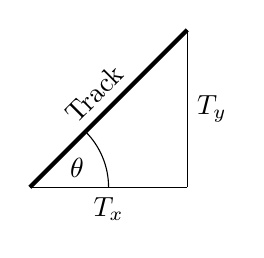
\begin{tikzpicture}
		\draw (0,0) -- node[below]{$T_x$} (2,0);
		\draw (2,0) -- node[right]{$T_y$} (2,2);
		\draw[line width=0.55mm] (2,2) -- node[above, rotate=45]{Track} (0,0);
		\draw (1,0) arc (0:45:1);
		\node at (0.6,0.25) {$\theta$};
		\end{tikzpicture}
		\caption{test}
	\end{minipage}
	\hspace{1cm}
	\begin{minipage}{0.45\textwidth}
		\centering
		\captionof{table}{test}
		\begin{tabular}{rrl}
			\toprule
			$T_x \ [\si{\meter}]$ & $T_y \ [\si{\meter}]$ & $\theta \ [\si{\radian}]$\\
			\midrule
			1.01 & 1.01 & $0.785 \approx \sfrac{\pi}{4}$\\
			1.16 & 0.83 & $0.621 \approx \sfrac{7\pi}{36}$\\
			1.275 & 0.64 & $0.465 \approx \sfrac{5\pi}{36}$\\
			1.37 & 0.42 & $0.297 \approx \sfrac{\pi}{12}$\\
			\bottomrule
		\end{tabular}
	\end{minipage}
\end{figure}

\begin{figure}[h]
	\begin{minipage}{0.45\textwidth}
		\centering
		\captionof{table}{Measurements of $\delta t$ and $(s_x)_f$ taken for the a launch angle of $\sfrac{\pi}{4}$}
		\begin{tabular}{crr}
			\toprule
			Trial No. & $\delta t \ [\si{\milli\second}]$ & $(s_x)_f \ [\si{\meter}]$\\
			\midrule
			1 & 48.01 & 1.025\\
			2 & 46.70 & 0.985\\
			3 & 44.60 & 1.010\\
			4 & 46.42 & 1.040\\
			\midrule
			Average & & \\
			\bottomrule
		\end{tabular}
	\end{minipage}
	\hspace{1cm}
	\begin{minipage}{0.45\textwidth}
		\centering
		\captionof{table}{Measurements of $\delta t$ and $(s_x)_f$ taken for the a launch angle of $\sfrac{7\pi}{36}$}
		\begin{tabular}{crr}
			\toprule
			Trial No. & $\delta t \ [\si{\milli\second}]$ & $(s_x)_f \ [\si{\meter}]$\\
			\midrule
			1 & 35.66 & 1.470\\
			2 & 35.16 & 1.485\\
			3 & 33.68 & 1.520\\
			4 & 34.04 & 1.525\\
			\midrule
			Average & & \\
			\bottomrule
		\end{tabular}
	\end{minipage}
\end{figure}

\begin{figure}[h]
	\begin{minipage}{0.45\textwidth}
		\centering
		\captionof{table}{Measurements of $\delta t$ and $(s_x)_f$ taken for the a launch angle of $\sfrac{5\pi}{36}$}
		\begin{tabular}{crr}
			\toprule
			Trial No. & $\delta t \ [\si{\milli\second}]$ & $(s_x)_f \ [\si{\meter}]$\\
			\midrule
			1 & 30.34 & 1.590\\
			2 & 30.39 & 1.540\\
			3 & 29.73 & 1.570\\
			4 & 29.94 & 1.575\\
			\midrule
			Average & & \\
			\bottomrule
		\end{tabular}
	\end{minipage}
	\hspace{1cm}
	\begin{minipage}{0.45\textwidth}
		\centering
		\captionof{table}{Measurements of $\delta t$ and $(s_x)_f$ taken for the a launch angle of $\sfrac{\pi}{12}$}
		\begin{tabular}{crr}
			\toprule
			Trial No. & $\delta t \ [\si{\milli\second}]$ & $(s_x)_f \ [\si{\meter}]$\\
			\midrule
			1 & 27.27 & 1.450\\
			2 & 26.79 & 1.425\\
			3 & 26.94 & 1.410\\
			4 & 26.92 & 1.405\\
			\midrule
			Average & & \\
			\bottomrule
		\end{tabular}
	\end{minipage}
\end{figure}

\newpage

\section{Calculations}
Equation (4) relies on a known force profile, applied to the object, to determine the launch velocity reached at the linear track termination. With some effort, the force could be found using detailed information about the electric motor dynamics and torque speed characterisitcs. A simpler method of calculating initial launch velocity magnitude would be to calculate average velocity over a short distance towards the track termination, and use this value as an approximate. If the short distance is denoted as $\Delta s$, and the time taken to traverse this distance is $\delta t$, then average velocity is calculated as:
\begin{equation}
v_{avg} = \frac{\Delta s}{\delta t}
\end{equation}

As outlined in Section XXXX, a small device of approximately $0.1\si{\meter}$ in length measures the time taken for the car to traverse this distance. Letting $\Delta s = 0.1\si{\meter}$, and using the average times calculated in Tables XXXX, XXXX, XXXX, and XXXX for $\delta t$, we can calculate the approximate launch velocity for each of the ramp angles. The results of these calculations can be found in Table XXXX.
\begin{figure}[h]
	\begin{minipage}{0.45\textwidth}
		\centering
		\captionof{table}{text}
		\begin{tabular}{ll}
			\toprule
			Angle $(\theta)$ & Velocity $(|\boldsymbol{v_0}|)$\\
			\midrule
			\bottomrule
		\end{tabular}
	\end{minipage}
	\begin{minipage}{0.45\textwidth}
		\centering
		\begin{tikzpicture}
			\begin{axis}
				[
				axis y line = middle,
				axis x line = middle,
				domain=0:5,
				xmin=0,xmax=6,
				ymin=0,ymax=5,
				ticks=none
				]
				\addplot[blue]{-0.5*(x*x-4*x-5)};
				\addplot[thick, red, ->, domain=0:1]{2.5+2*x};
				\addplot[domain=0:1]{2.5};
			\end{axis}
			\node[left] (a) at (0,2.8) {$(s_y)_0$};
			\node[below] (b) at (5.8,0) {$(s_x)_f$};
			\node[red,above] (b) at (1.3,5) {$\boldsymbol{v_0}$};
			\node[above] (b) at (0.32,2.82) {$\theta$};
		\end{tikzpicture}
		\caption{text}
	\end{minipage}
\end{figure}

Suppose the initial velocity $\boldsymbol{v_0}$, launch angle $\theta$, and launch height $(s_0)_y$ are known. The initial velocity can be decomposed into $x$ and $y$ components as follows:
\begin{align}
(v_x)_0 &= |\boldsymbol{v_0}|\cos(\theta)\\
(v_y)_0 &= |\boldsymbol{v_0}|\sin(\theta)
\end{align}

To find the horizontal distance, $(s_x)_f$, at the point of projectile impact we can employ the known equation of motion for $s_x(t)$ shown in Table 1. In order to calculate $(s_x)_f$ using this equation, we first need to determine the time taken for the object to collide with the ground. This can be found using the equation for vertical displacement, $s_y(t)$, also shown in Table 1. Specifically, we are interested in the case when $s_y(t) = 0$. This yields the following:
\begin{equation}
0 = (s_y)_0 + (v_y)_0 t - \frac{1}{2}gt^2
\end{equation}

Multiplying equation (XXXX) throughout by 2, and solving using the quadratic formula yields:
\begin{equation}
t = \frac{2(v_y)_0 \pm \sqrt{4(v_y)_0^2 + 8g(s_y)_0}}{2g}
\end{equation} 

Noting that $2(v_y)_0 < \sqrt{4(v_y)_0^2 + 8g(s_y)_0}$ and $t>0$ we can discard on solution. Hence, when $(s_y(t) = 0)$, we note that:
\begin{equation}
t = \frac{2(v_y)_0 + \sqrt{4(v_y)_0^2 + 8g(s_y)_0}}{2g}
\end{equation}

Now, to find $(s_x)_f$ we can substitute the expression for time in (14) to the equation of horizontal displacement, $s_x(t)$, from Table XXXX. This will gives us the following:
\begin{equation}
(s_x)_f = (s_x)_0 + \frac{(v_x)_0}{2g} \bigg[2(v_y)_0 + \sqrt{4(v_y)_0^2 + 8g(s_y)_0}\bigg]
\end{equation}

Noting that, by design, our coordinate system assignment ensures that $(s_x)_0 = 0$, hence, equation (15) simplifies to:
\begin{equation}
(s_x)_f = \frac{(v_x)_0}{2g} \bigg[2(v_y)_0 + \sqrt{4(v_y)_0^2 + 8g(s_y)_0}\bigg]
\end{equation}

Equation (16) has been applied to each of the four launch angles. The important parameters here are: $\boldsymbol{v_0}$, $\theta$, and $(s_y)_0$. The calculation results can be seen in Table XXXX. The table also shows the measured result and the error between actual and predicted denoted as $\epsilon$.
\begin{table}[h]
	\centering
	\caption{text}
	\begin{tabular}{rrrrr}
		content...
	\end{tabular}
\end{table}

\section{Discussion}


\section{Conclusion}

\bibliography{my_bib}
\bibliographystyle{ieeetr}

\end{document}